
\documentclass[a4paper,12pt]{book}
\usepackage{tabularx}
\usepackage[a4paper, left=1in,right=1in,top=2cm,bottom=1.5cm]{geometry}
\usepackage{fancyhdr}
\usepackage{csvsimple}
\pagestyle{plain}
\renewcommand{\chaptername}{Experiment}
\usepackage[utf8]{inputenc}
\usepackage{pdfrender}
\usepackage{xcolor}
\usepackage{ae}
\usepackage{multirow}
\usepackage{aecompl}
\usepackage{helvet}
\usepackage{afterpage}
\usepackage{graphicx}
\usepackage{caption}
\usepackage{array}
\usepackage{subcaption}
\makeatletter
\newcommand\@addfig{\relax}
\newcommand\addfig[1]{\global\long\def\@addfig{#1}}
\newcommand\@putfig{\@addfig\addfig{\relax}}
\newcommand\blankpage{%
	\null
	\vfill
	\@putfig%
	\vfill
	\thispagestyle{empty}% BEWARE, if you want the header and footer, you should put the correct style here
	\clearpage%
	\addtocounter{page}{-1}% BEWARE, if you want the left pages to be numbered, don't put this line, this is intended to have picture page with the same number as the facing text page
	\afterpage{\blankpage}}
	\makeatother

	\begin{document}
	%\pdfrender{StrokeColor=black,TextRenderingMode=2,LineWidth=0.1pt}
	\afterpage{\blankpage}
	%-------Hematology----{{{
	\part{Hematology}
	%-------CompoundMicroscope---{{{
	\chapter*{\centering Compound Microscope}

	\begin{tabular}{p{5in} p{1in}}
		\textbf{Exp No:}  & \textbf{Date:}\\
	\end{tabular}
	\section*{Introduction}
	\par
	A microscope is an optical instrument which magnifies the image of an object.
	There are various types of microscope which use different types of lens and different principles of optics.
	Compound microscope is one of the most frequently used equipment in a medical laboratory.\newline

	\addfig{%
		\begin{figure}[h]
			\centering
			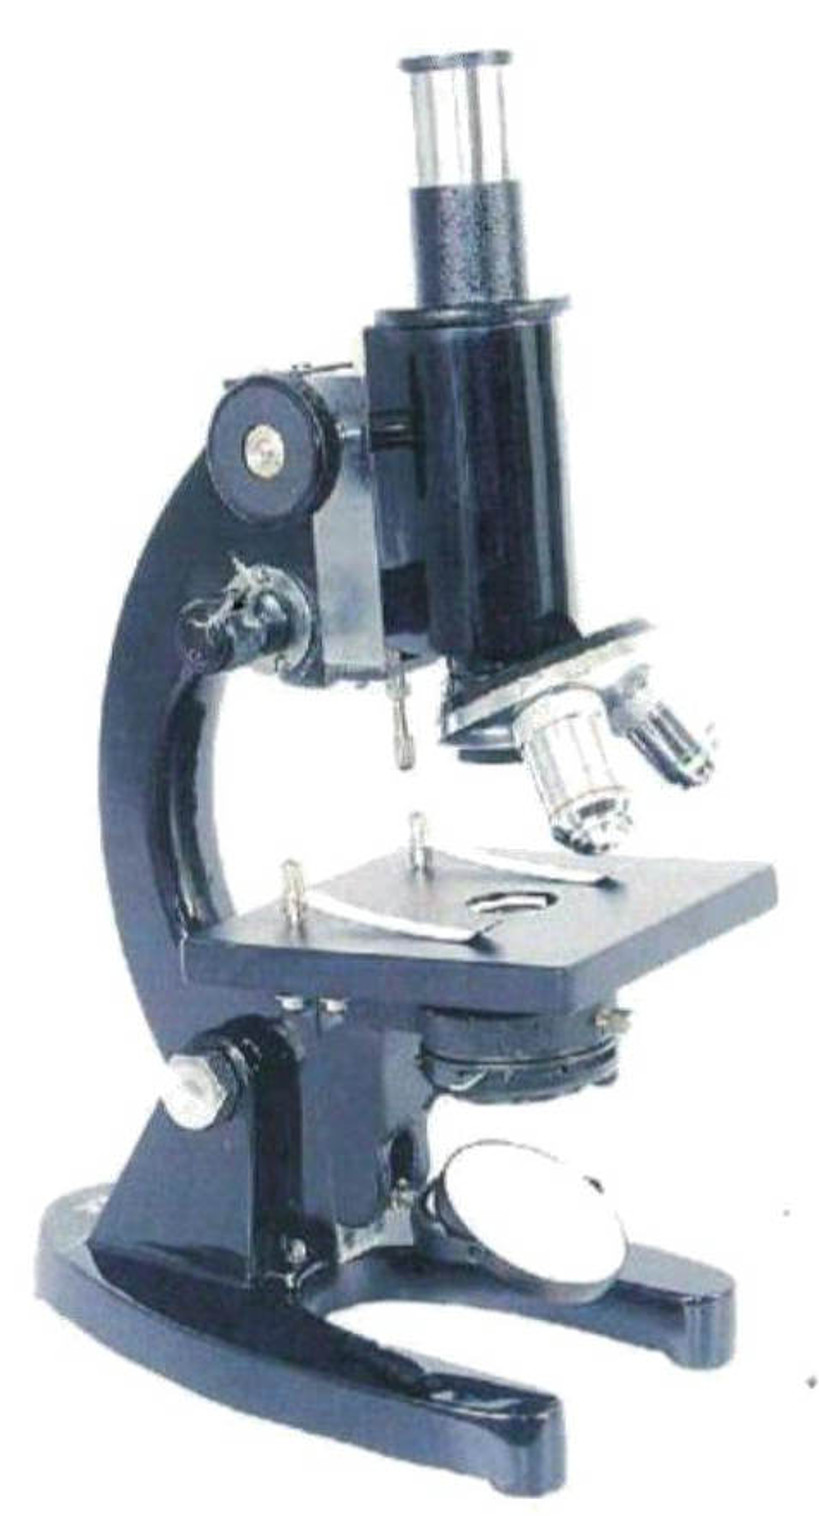
\includegraphics[scale=10]{./compoundMicroscope.jpg}
			\caption*{\textbf{Compound Microscope}}
			\label{compound microscope}
		\end{figure}
		}

		Physical terms:
		\begin{itemize}
			\item{Resolution \par It is the ability to reveal closely adjacent structural details as separate and distinct. The limit of magnification of a microscope is set by its resolving power.}
			\item{Numerical Aperture \par It is the ratio of the diameter of the lens to its focal length. Greater the numerical aperture greater the resolving power.}
			\item{Working Distance \par It is the distance between the objective lens and the slide.}
		\end{itemize}

		\section*{Parts Of The Microscope}

		\subsection*{Support System}
		\begin{enumerate}
			\item{Base \par It supports the microscope on the working table.}
			\item{Pillars \par Two upright pillars project upwards from the base.}
			\item{Handle \par Handle is hinged to the pillars. It supports the magnifying and adjusting systems. It is the handle by which the microscope must be carried. It is curved and the microscope can be tilted at the hinged joint.}
			\item{Body tube \par The eyepiece fits into the top of the body tube. The nose piece with the objective lenses fits into its lower end. It is the part through which the light passes to the eyepiece. It actually conducts the image.}
			\item{Stage \par Fixed stage is the horizontal platform on which the object is placed. It has a central opening through which the illuminating system focuses the light on the object. Mechanical stage has a spring mounted clip to hold the slide or counting chamber in position. It has two screws to move the mounted object from side to side and for ward and backwards.}
			\item {Nose piece \par Fixed nose piece is attached to lower end of body tube. Revolving nose piece carries objective lenses of different magnifying powers.}
		\end{enumerate}

		\subsection*{Adjusting System}
		It consists of the coarse and fine adjustment screws mounted in the handle by a double sided micrometer mechanism.
		\begin{enumerate}
			\item{Coarse adjustment screws \par It consists of rack and pinion which moves the tube rapidly through a large distance when the screw is rotated clockwise or anticlockwise. It is used to obtain an approximate focus of the object.}
			\item{Fine adjustment screws \par Similar to coarse adjustment screw, but several rotations will move the tube through a very small distance. It is used to obtain exact focus of the object.}
		\end{enumerate}

		\subsection*{Illumination System}
		\begin{enumerate}

			\item{Source of illumination \newline
				\par Light source may be internal or external.
				\par Internal source –In modern microscopes, there is an in-built light source with an electrical tungsten lamp, which is placed directly under the stage.
				\par External source – This can be from an electric lamp housed in a lamp box with a window or from the sun. The rays of light are reflected by a mirror towards the object. The mirror is located at the base of the microscope which is plain or concave.}
			\item{Condenser
				\par It focuses the rays of light reflected from the mirror onto the object under observation and helps in resolving the image. It is mounted below the stage of the microscope. Position of the condenser has to be adjusted according to the objective lens used.}
			\item{Iris diaphragm
				\par It is located at the bottom of the condenser. It has a central aperture. The size of the aperture can be altered to regulate the amount of light that passes through the condenser onto the object under observation.}
		\end{enumerate}

		\subsection*{Magnification System}
		\begin{enumerate}

			\item{Eye piece
				\par This is a magnifying lens inserted into the upper end of the body tube. Each eyepiece has two lenses, an eye lens mounted at the top and a field lens at the bottom. It has a magnification power of 5 and 10. It magnifies the primary image to give a virtual image which is observed through the eye piece.}
			\item{Objective lens

				\par Three objective lenses are fitted to the lower end of the body tube in the revolving nose piece. They are the low power, high power and oil immersion objective lenses. The desired objective lens is placed close to object on the stage and it produces a real magnified and inverted primary image. When the oil immersion objective is used, the space between the object and the lens is filled with cedar wood oil which has the same refractive index as that of glass and hence prevents refraction of light.\newline
				\begin{tabular}{c | c | c | c}
					\hline
					Objective & Working Distance & Numerical Aperture &Magnification\\
					\hline
					Low Power & 5 to 15 millm & 0.3 & 10\\
					\hline
					High Power
					&0.5 to 4 millm
					&0.65
					&40/45 \\
					\hline

					%next row
					Oil immersion
					&0.15 to 1.5 millm
					&1.3
					&100 \\

					\hline





				\end{tabular}

				\par
				Adjustments for low power objective
				\begin{itemize}
					\item {Concave mirror is used.}
					\item {Condenser is lowered.}
					\item {Iris diaphragm is slightly opened to decrease the intensity of illumination.}
				\end{itemize}

				\par
				Adjustments for high power objective
				\begin{itemize}
					\item{Concave mirror is used.}

					\item{Condenser is slightly raised.}

					\item{Iris diaphragm is partially opened to increase the intensity of illumination.}
				\end{itemize}

				\par
				Adjustments for oil immersion objective (OPR)
				\begin{itemize}

					\item{Open the Iris diaphragm fully to get maximum intensity of illumination}

					\item{Plane mirror is used.}

					\item{Raise the Condenser.}
				\end{itemize}
				}




			\end{enumerate}

			\section*{Precautions}
			\begin{itemize}
				\item Objectives and eyepiece should be free from dust.
					item The mirror, the position of the condenser, and the aperture of the iris should be checked in order to get proper illumination.
				\item While changing the objective it should be noted that the objective clicks into its proper position.
				\item Do the necessary microscopic adjustments before using each objective.
				\item While focusing, lower the objective close to the slide and focus the object by slowly raising the objective.
				\item Never bring down the objective with the coarse adjustment screw while looking into the microscope.
				\item Examine the slide under low power and high power before examining it under oil immersion objective.
				\item After using oil immersion objective, clean the lens with filter paper and xylol.
			\end{itemize}

			\section*{Questions}
			\begin{enumerate}
				\item Name the oils used for oil immersion objective.
				\item How will you calculate the total magnification power of the microscope for each objective?
				\item Name the other types of microscope.
			\end{enumerate}
			%------}}}
			%-----------Hemocytometer----{{{

			\chapter*{\centering Hemocytometer}
			\begin{tabular}{p{5in} p{1in}}
				\textbf{Exp No:}  & \textbf{Date:}\\
			\end{tabular}

			\addfig{%
				\begin{figure}[h]
					\centering
					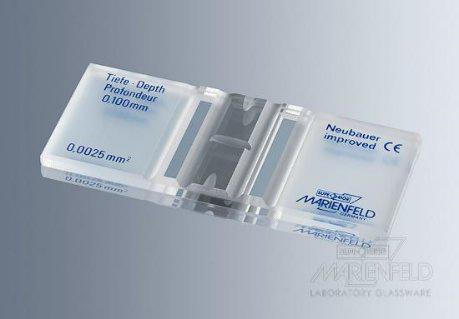
\includegraphics[scale=.5]{./neubar.jpg}
					\caption*{\textbf{Neubauer Chamber}}
					\vspace{1.5cm}
					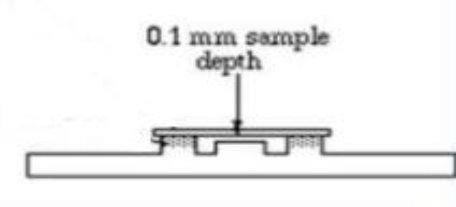
\includegraphics[scale=0.5]{./neubarSide.jpg}
					\caption*{\textbf{Neubauer Chamber - side view}}
					\vspace{2cm}
					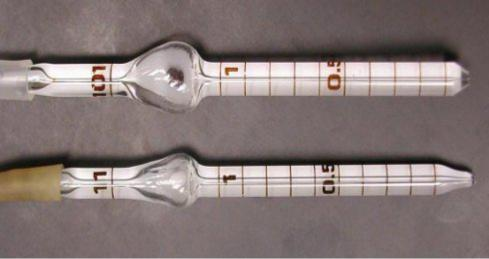
\includegraphics[scale=.5]{./pipette.jpg}
					\caption*{\textbf{RBC \& WBC pipettes}}
					\label{chamber}
				\end{figure}
				}
				\addfig{%
					\begin{figure}[h]
						\centering
						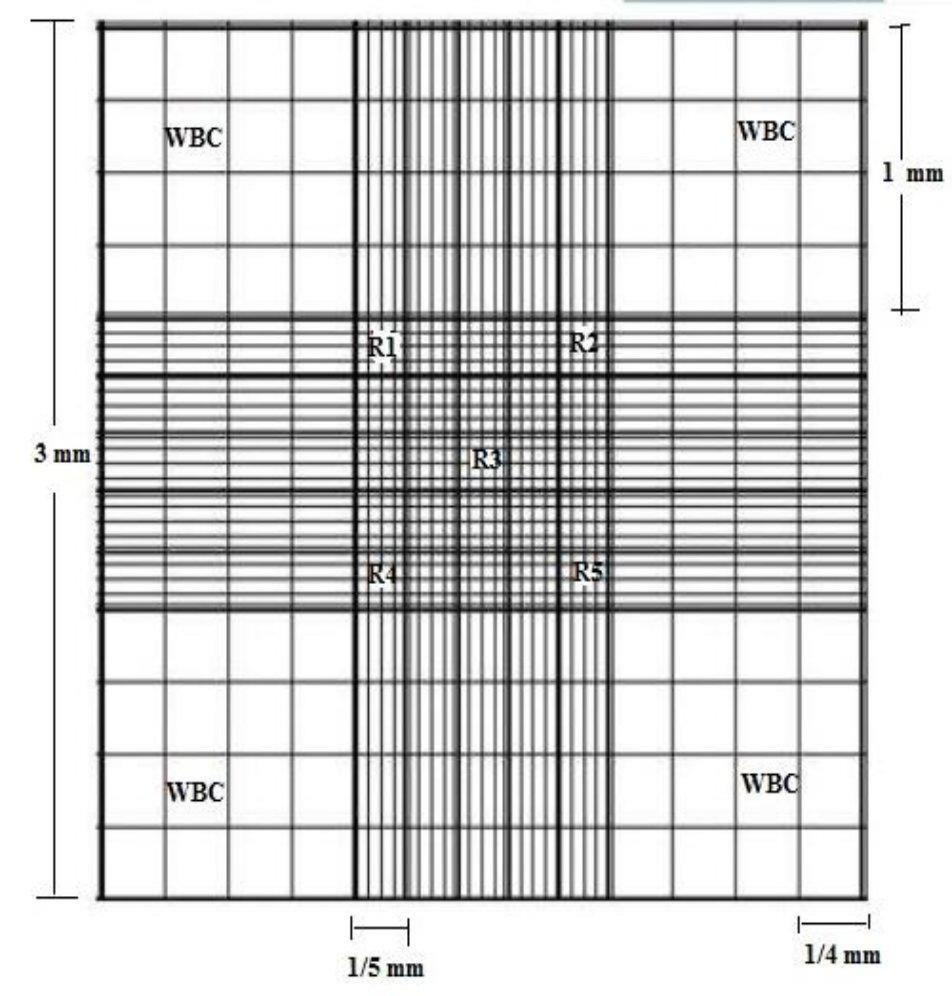
\includegraphics[scale=.5]{./grid.jpg}
						\caption*{\textbf{Neubauer Chamber's Counting Region}}
						\label{grid}
					\end{figure}
					}


					\section*{Introduction}
					The formed elements of blood are counted by Hemocytometry. The apparatus is called as hemocytometer. It consists of diluting pipettes and counting chamber.
					The counting chamber in common use is the improved Neubauer’s counting chamber. This is a thick glass slide divided into two central platforms by a ‘H’ shaped groove. The central platform is slightly lower than the sides. When a cover slip is placed over the central platforms, resting on the side platforms, a space of $\frac{1}{10}$  $mm$ depth will be present between the cover slip and the central platform. This area is used for charging the chamber with the diluted blood for cell counting.
					The central platforms have ruled squares which are used for cell counting. The ruled area is a square measuring 3 $mm$ $\times$ 3 $mm$. This area is divided into 9 large equal squares each having an area of 1 $mm$$^2$. The four large corner squares are used for WBC count. The central square is used for RBC count. All nine squares are used for Absolute eosinophil count.

					\section*{WBC counting squares}
					\begin{itemize}
						\item
							The four large corner squares are used for the WBC count and each has 16 medium squares (16$\times$4=64 medium squares).
						\item {
								Side of each large square is 1 $mm$.}
							\item{
									Area of each large square is 1 $\times$ 1 = 1 $mm$$^{2}$.}
								\item {
										Volume of each large square = area $\times$ depth = 1 $\times$ $\frac{1}{10}$ = $\frac{1}{10}$ $mm^3$.}
								\item{
										Volume of each medium square = $\frac{1}{4}$ $\times$ $\frac{1}{4}$ $\times$ $\frac{1}{10}$ = $\frac{1}{160}$ $mm^3$.}
					\end{itemize}

					\section*{RBC counting squares}
					\begin{itemize}

						\item{The 1$mm^2$ central RBC square is divided into 25 medium sized squares by triple lines. The four corner and central medium sized squares are used for RBC count.}
						\item{Each medium sized square is further divided into 16 small squares.}
						\item{(5 $\times$ 16 = 80 small squares).}
						\item{Side of each medium sized square is $\frac{1}{5}$ $mm$.}
						\item{Area of each medium sized square is $\frac{1}{5}$ $\times$ $\frac{1}{5}$ = $\frac{1}{25}$ $mm^2$.}
						\item{Volume of each medium sized square is $\frac{1}{250}$ $mm^3$.}
						\item{Volume of each smallest square = $\frac{1}{20}$ $\times$ $\frac{1}{20}$ $\times$ $\frac{1}{10}$ = $\frac{1}{4000}$ $mm^3$.}

					\end{itemize}

					\section*{Pipettes}
					The pipettes are used to dilute the blood to a known dilution.
					Two types of pipettes are used – RBC pipette, WBC pipette .
					\par


					Parts of a pipette are:-\newline
					\textbf{The Stem:}
					The long narrow stem has a capillary bore and a well-grounded conical tip. It is divided into 10 equal parts with two numbers etched on it – 0.5 in the middle and 1.0 at the junction of stem and the bulb.\newline
					\textbf{The bulb:}
					The bulb contains a free-rolling bead. The bead helps in identifying the pipette and mixing the diluents with blood in the bulb. Free rolling of the bead in the bulb indicates whether the pipette is dry or not.\newline
					\textbf{Rubber tube and mouthpiece:}
					The narrow rubber tube attached to the bulb, facilitates filling of the pipette by gentle suction. There is a marking just above the bulb. This marking is 11 in WB C pipette and 101 in RBC pipette. The graduations do not indicate absolute or definite amounts in terms of cubic mm .They only indicate relative volumes in relation to each other. The markings indicate relative parts in the pipette\newline

					\subsection*{RBC pipette}
					\begin{itemize}

						\item{Markings are 0.5, 1.0 and 101}
						\item{The capillary bore is narrow}
						\item{Bulb is larger and has a red bead}
						\item{Volume of the bulb is 100 parts}
					\end{itemize}

					\subsection*{WBC pipette:}
					\begin{itemize}
						\item{Markings are 0.5, 1.0 and 11}
						\item{The capillary bore is wider}
						\item{Bulb is smaller and has a white bead}
						\item{Volume of the bulb is 10 parts}
					\end{itemize}


					\subsection*{Finger Prick}
					\begin{itemize}
						\item{Clean the tip of the finger with spirit and allow the area to dry.}
						\item{Prick the tip of finger with the lancet, deep enough to get a good drop of blood.}
						\item{Don’t squeeze the finger pulp after pricking as this leads to the seepage of tissue fluid resulting in dilution of the blood.}
						\item{The prick is usually made on middle or ring finger.}
					\end{itemize}

					\subsection*{Filling The Pipette}
					\begin{itemize}

						\item{Under aseptic precautions prick the finger and wipe away the first drop and allow the flowing blood to form a good sized drop.}
						\item{Hold the pipette horizontally and dip its end into the blood drop. Gently suck blood upto 0.5 or 1.0 mark depending on the dilution required.}

						\item{If the blood overshoots 0.5 or 1.0 mark, remove the excess blood by gently tapping the tip of the pipette on to the palm. Do not use cotton or any absorbent material as it might absorb water content of blood and concentrates blood.}
						\item{Place the tip of the pipette into the diluting fluid and suck upto the 11 mark in case of WBC pipette or 101 mark in case of RBC pipette without any air bubble.}
						\item{Place the pipette horizontally between the palms of both hands with the rubber tube folded parallel to it and roll the pipette for 1-2 minutes, for thorough mixing of blood with the fluid in the bulb.}

					\end{itemize}

					\subsection*{Precautions}
					\begin{itemize}

						\item{The pipette must be dry and free from clotted blood and the bead must roll freely in the bulb.}
						\item{The tip must not press against the finger or be lifted out of the blood drop or else air will enter it.}
						\item{The blood must be diluted immediately, or else it may clot.}
						\item{Always hold the pipette horizontally to avoid leakage of fluid from the pipette while mixing.}

					\end{itemize}


					\subsection*{Focussing The Counting Grid}
					\begin{itemize}

						\item{	Focus the counting grid with low power and then high power objective.}
						\item{	The lines of the squares must be seen clearly.}
					\end{itemize}

					\subsection*{Charging The Chamber}
					\begin{itemize}

						\item{	 Place the coverslip on the central platform of the chamber covering the ruled squares.}
						\item{	 Discard the stem fluid before charging the chamber as it contains only the diluting fluid.}
						\item{	 Form a good drop of diluted blood at the tip of the pipette, by squeezing the rubber tube, while closing its mouthpiece or by gently blowing through the rubber tube.}
						\item{	 Hold the pipette at 45 degree inclination and touch the chamber with the  tip of the pipette between the cover slip and the central platform.}
						\item{	 A thin layer of the fluid spreads under the coverslip on the central  platform by capillary action.}
						\item{	 Avoid overcharging the chamber which is recognized by fluid in the  trenches.}
						\item{	 Wait for 2 minutes for the cells to settle down.}
						\item{	 Focus  the  squares  under  the  desired  objective  and  start  counting.}
					\end{itemize}


					\subsection*{Precautions}
					\begin{itemize}

						\item{	 The chamber and the coverslip should be properly cleaned.}
						\item{	 The contents of the bulb must be thoroughly mixed before charging.}
						\item{	 2-3 drops of fluid must be discarded from the pipette before charging as the stem contains only diluents.}
						\item{	 Air bubbles should not enter the platform of the chamber while charging.}
						\item{	 The chamber should not be overcharged ( gives false low results) or undercharged ( the cells may not be found in peripheral squares).}
					\end{itemize}

					\subsection*{Cell Counting}
					\begin{itemize}

						\item{	 Count the cells in the respective squares.}
						\item{	 Care should be taken not to count the same cells again by following L rule. (Count the cells present inside the square and those on the left and lower lines. Ignore those on the right and upper lines).}
					\end{itemize}

					\subsection*{Questions}

					\begin{enumerate}

						\item{	 What are the other types of cell counting chambers ?}

						\item{	 What are the other cells that can be counted using Neubauer’s chamber?}
						\item{	 Mention the differences between RBC and WBC pipettes.}
					\end{enumerate}
					%-----------}}}
					%-------RBCcount---{{{
					\chapter*{\centering Estimation Of Total RBC Count}

					\begin{tabular}{p{5in} p{1in}}
						\textbf{Exp No:}  & \textbf{Date:}\\
					\end{tabular}

					\section*{Aim}

					To enumerate the number of  erythrocytes in 1 $mm^3$ of blood.
					\section*{Apparatus Required}
					Microscope, Hemocytometer (RBC diluting pipette and counting chamber), RBC diluting fluid (Hayem’s fluid), spirit, cotton and lancet.

					\section*{Hayem's Fluid - composition}
					\begin{itemize}

						\item{		Sodium chloride - 0.5 g	- Maintains isotonicity}
						\item{		Sodium bisulphate - 2.5 g - Prevents aggregation  of RBCs (Rouleaux formation)}
						\item{		Mercuric perchloride - 0.25 g - Acts  as preservative, antifungal and antibacterial}
						\item{		Distilled water - 100 ml - Acts as solvent}
					\end{itemize}


					\section*{Procedure}

					Make  a  sterile  finger  prick  and  discard  the  first drop  of blood. Draw blood upto  0.5  mark  and  Hayem’s  fluid  upto 101  mark  with  the  pipette. Mix  the contents thoroughly. Discard  the  first  few  drops and then charge  the  Neubauer chamber. Allow  the cells to  settle  for  3-4  minutes.Count the RBCs in the 4 medium sized corner squares and  in the central medium sized square of the RBC counting area (total of 16 x 5 = 80 smallest squares) under high power objective.


					\section*{Calcualtion}
					Number of RBCs in 5 medium sized RBC squares = n\newline\vspace{.4cm}
					Area of 1 medium  sized RBC square =$\frac{1}{5}$ $\times$ $\frac{1}{5}$ = $\frac{1}{25}$ $mm^2$\newline\vspace{.4cm}
					Volume of 1 medium sized RBC square = $\frac{1}{25}$ $\times$ $\frac{1}{10}$ = $\frac{1}{250}$ $mm^3$\newline\vspace{.4cm}
					Volume of 5 medium sized RBC squares = $\frac{1}{250}$ $\times$ 5= $\frac{1}{50}$ $mm^3$\newline\vspace{.4cm}
					Number of cells in  $\frac{1}{50}$ $mm^3$ of diluted blood  = n\newline\vspace{.4cm}
					Number of cells in  1 $mm^3$  of diluted blood = 50 n\newline\vspace{.4cm}
					Dilution factor = 1 : 200\newline\vspace{.4cm}
					Number of cells in 1 $mm^3$ of un diluted blood 	= n $\times$ 50 $\times$ 200  \newline\vspace{.4cm}

					\section*{Result}
					RBC  count in the given  blood sample is $\rule{5cm}{0.1cm}$ cells / $mm^3$
					\section*{Questions}
					\begin{enumerate}

						\item {Name the other diluting fluids used for red  cell count.}
						\item{How will you identify the RBC counting squares?}
						\item{What is the normal RBC count in males and females?}
						\item{Why is the RBC count high in males?}
						\item{Mention the physiological and pathological causes for anemia and polycythemia?}


					\end{enumerate}
					%-----------}}}
					%--------WBC count---{{{
					\chapter*{\centering Estimation Of Total WBC Count}

					\begin{tabular}{p{5in} p{1in}}
						\textbf{Exp No:}  & \textbf{Date:}\\
					\end{tabular}
					\section *{Aim}
					To enumerate the number of leucocytes (white blood cells) in 1 $mm^3$ of blood.
					\section*{Apparatus Required}
					Microscope, Hemocytometer, WBC pipette, Turk’s fluid, Spirit, Cotton, Lancet
					\section*{Turk's Fluid Composition}
					\begin{tabular}{l c l}

						1\% Glacial Acetic Acid	&	-&	1.5 ml - Lyses RBCs without affecting WBCs\\
						Gentian Violet&			-&	1.5 ml - Stains nuclei of WBCs\\
						Distilled Water&		-&	100 ml - Acts as solvent\\

					\end{tabular}
					\section*{Procedure}

					Make a sterile finger prick and discard the 1st drop of blood. Draw blood upto 0.5 mark and Turk’s fluid upto 11 mark in the WBC pipette. Mix the contents thoroughly. Discard the first few drops and charge the Neubauer chamber. Allow the cells to settle for 3 to 4 minutes. Count the WBCs in the 4 corner large squares (WBC counting area) under high power objective.

					\section*{Calcualtion}

					Number of cells in 4 WBC squares = n\newline\vspace{.2cm}
					Area of 1 WBC square = 	1$\times$ 1 	= 1 $mm^2$\newline\vspace{.2cm}
					Volume of 1 WBC square	= 1$\times$ $\frac{1}{10}$ = $\frac{1}{10}$ $mm^3$\newline\vspace{.2cm}
					Volume of 4 WBC squares =4$\times$ $\frac{1}{10}$ = $\frac{4}{10}$ $mm^3$\newline\vspace{.2cm}
					Number of cells in $\frac{4}{10}$ $mm^3$ of Diluted blood 	= n \newline\vspace{.2cm}
					Therefore, Number of cells in 1 $mm^3$ of Diluted blood = 	n $\times$ $\frac{10}{4}$\newline\vspace{.2cm}
					Dilution Factor = 1 : 20\newline\vspace{.2cm}
					Therefore, Number of cells in 1 $mm^3$ of Undiluted blood 	= n $\times$ $\frac{10}{4}$ $\times$ 20 =	n $\times$ 50\newline\vspace{.2cm}


					\section *{Result}

					WBC count in the given  blood sample is $\rule{5cm}{0.1cm}$ cells / $mm^3$

					\section*{Questions}


					\begin{enumerate}

						\item{What is the normal RBC : WBC ratio ?}
						\item{ In which condition is RBC pipette used for counting WBCs ?}
						\item{ Why is blood diluted only 20 times in WBC counting?}
						\item{ Mention the physiological and pathological causes of high and low WBC count.}
						\item{ What is Leucocytosis ?}
						\item{ What is Leukemia?}
					\end{enumerate}
					%----}}}
					%------AEC---{{{
					\chapter*{\centering Absolute Eosinophil Count}

					\begin{tabular}{p{5in} p{1in}}
						\textbf{Exp No:}  & \textbf{Date:}\\
					\end{tabular}

					\section*{Aim}

					To determine the number of eosinophils per cu mm of blood
					\section*{Apparatus Required}
					Microscope, Hemocytometer, Dunger’s fluid, spirit, cotton and lancet.
					\section*{Dunger's Fluid Composition}
					1\% of solution of eosin in water (5$ml$)- Eosin stains the eosinophilic granules.\newline
					Acetone (5$ml$) - Acetone lyses the cell membrane of all other cells.\newline
					Distilled water (90$ml$) - Distilled water to make up to 100$ml$.Acts as solvent.\newline
					\section*{Procedure}
					Make a sterile finger prick and discard the first drop of blood. Draw blood upto 1 and the Dunger’s fluid upto mark 11 in a WBC pipette. Mix the contents thoroughly. Cover the pipette with a petri dish lined by moistened filter paper. Wait for 15 minutes. Discard the first few drops and charge the Neubauer chamber. The eosinophils are identified by the pinkish orange stained coarse granules in the cytoplasm. Count the Eosinophils in all the 9 large squares of the Neubauer chamber. Count within 30 minutes of charging .
					\section*{Calcualtion}
					Number of cells counted in 9 large squares				=	n\newline\vspace{.2cm}
					Area of 1 large square				=	1 $\times$ 1		=	1$mm^2$	\newline\vspace{.2cm}
					Volume of 1 large square				=	1 $\times$ $\frac{1}{10}$	=	$\frac{1}{10}$ $mm^3$\newline\vspace{.2cm}
					Volume of 9 large square				=	9 $\times$ $\frac{1}{10}$	=	$\frac{9}{10}$ $mm^3$\newline\vspace{.2cm}
					Number of cells in $\frac{9}{10}$ $mm^3$ of diluted blood				=	n\newline\vspace{.2cm}
					Number of cells in 1 $mm^3$ of diluted blood				=	n $\times$ $\frac{10}{9}$\newline\vspace{.2cm}
					Dilution factor								=	1:10\newline\vspace{.2cm}
					Therefore, number of cells in 1 $mm^3$ of undiluted blood		=	n$\times$$\frac{10}{9}$$\times$10
					=	n$\times$$\frac{100}{9}$
					\section*{Result}

					Abosolute Eosinophil count in the given  blood sample is $\rule{5cm}{0.1cm}$ cells / $mm^3$

					\section*{Questions}
					\begin{enumerate}

						\item{What is the normal value of Absolute Eosinophil Count ?}
						\item{What is the difference between the Differential Count and the Absolute Eosinophil Count ?}
						\item{What are the other diluting fluids used for Absolute Eosinophil Count?}
						\item{What are the contents of eosinophilic granules ?}
						\item{What are the functions of eosinophils?}
						\item{What are eosinopenia and eosinophilia?}
					\end{enumerate}
					%-----}}}
					%-----DC{{{
					\chapter*{\centering Diffrential Count}
					\begin{tabular}{p{5in} p{1in}}
						\textbf{Exp No:}  & \textbf{Date:}\\
					\end{tabular}

					\section*{Aim}
					To determine the differential count of White Blood Cells.
					\section*{Apparatus Required}
					Grease free and dry glass slides, Leishman’s stain, distilled water, lancet, spirit, cotton.	
					\section*{Leishman's Stain Composition \& Functions}
					Methylene blue (basic) 	     -	Stains acidic granules in cytoplasm especially 						granules of basophils and Nuclei of leucocytes.\newline
					Eosin (acidic) 		     -	Stains cytoplasm, basic granules in 							cytoplasm, Hemoglobin of RBCs.\newline
					Acetone free methyl alcohol - 	Fixes the cells (Acetone free methyl alcohol 						is used as acetone is a lipid solvent that 		lyses cell membrane).\newline 

					\section*{Procedure}

					\addfig{%
						\begin{figure}[h]
							\centering
							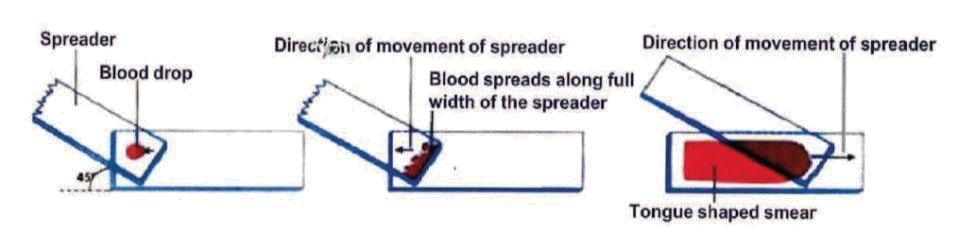
\includegraphics[scale=.50]{./smear1.jpg}
							\label{smear1}
							\vspace{3cm}
							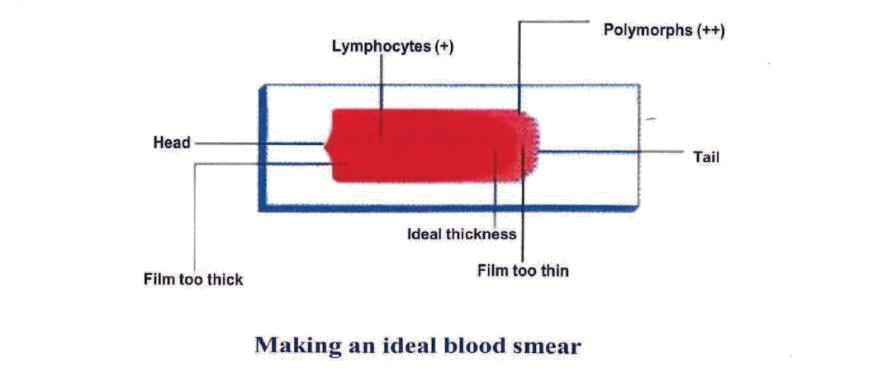
\includegraphics[scale=.50]{./smear2.jpg}
							\label{smear2}
							\vspace{1cm}
							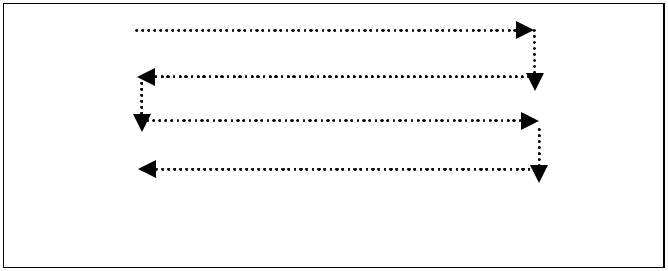
\includegraphics[scale=.50]{./smear3.jpg}
							\label{smear3}
						\end{figure}
						}
						Under aseptic precautions, prick the finger. Discard the first drop of blood. Place the slide on the table and support with left hand. Place the blood drop on the right end, one cm away from the edge. Place the spreader slide just infront of the blood drop. Draw the spreader slide backwards to touch the drop. The blood spreads across the edge of the spreader. Draw the spreader slide forward at an angle of 45$^{\circ}$ with a smooth, fast and firm movement to make a thin tongue shaped blood smear. Too thick, thin or a patchy smear is to be avoided. Air dry the smear quickly.

						Place the glass slide with the smear on a tray and add Leishman’s stain, drop by drop till the entire smear is covered with the stain. Count the number of drops added. Note the time and wait for 2 minutes (Fixation time). After 2 minutes, add double the quantity of distilled water over the film using a dropper. See to that the distilled water uniformly covers the entire surface of the slide and dilutes the stain homogenously. Gently blow the stain and the distilled water from one end of the slide to the other for uniform mixing. Wait for about 8-10 minutes for the smear to take up the stain uniformly (Staining time).
						Flush the slide under a gentle stream of tap water to remove the excess stain. Dry the slide. Scan the film under low \& high power objective. Make necessary microscopic adjustments for oil immersion objective (100X). Add a drop of cedar wood oil over the smear at the junction between the body and the tail, as the smear will be of one cell thickness with uniform staining here. Cedar wood oil has the same refractive index as that of glass and minimizes refraction. Examine in a zig-zag manner as shown in the figure.

						Draw a table with 100 squares to count 100 WBCs and enter the type of cell as identified while examining the film.

						\addfig{%
							\begin{figure}[h]
								\centering
								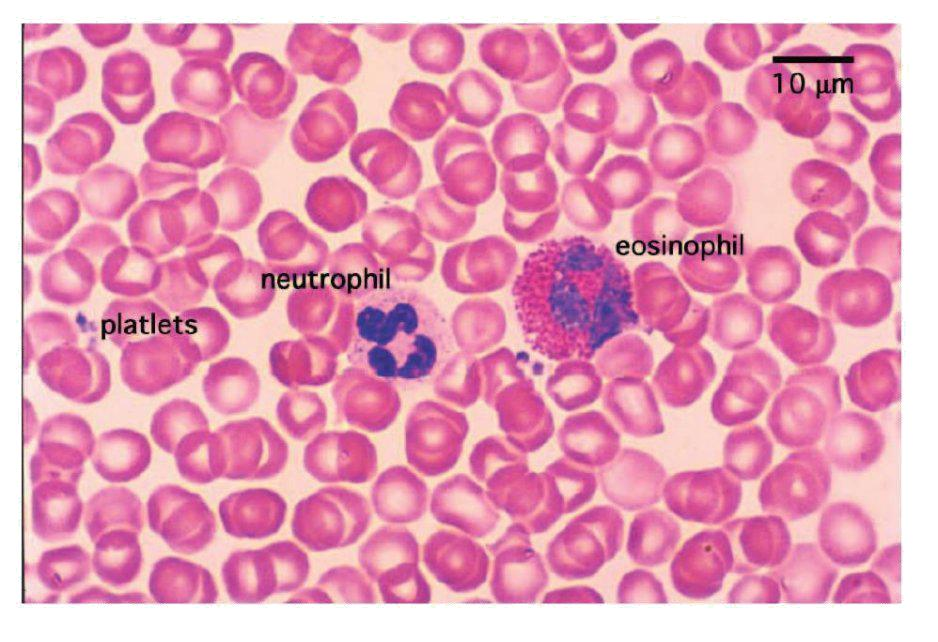
\includegraphics[scale=13]{./dc1.jpg}
								\label{dc1}
								\vspace{3cm}
								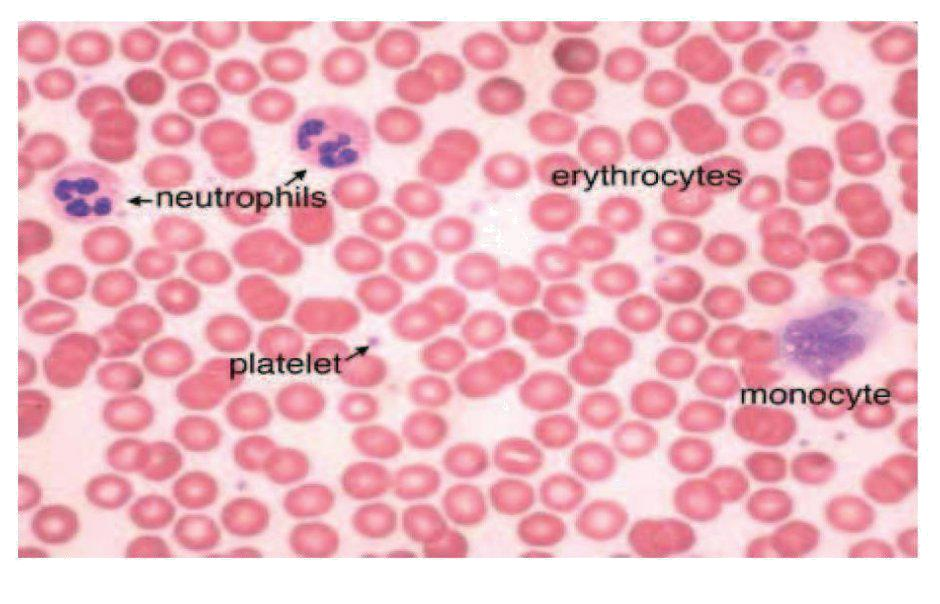
\includegraphics[scale=13]{./dc2.jpg}
								\label{dc2}
							\end{figure}
							}
							Under aseptic precautions, prick the finger. Discard the first drop of blood. Place the slide on the table and support with left hand. Place the blood drop on the right end, one cm away from the edge. Place the spreader slide just infront of the blood drop. Draw the spreader slide backwards to touch the drop. The blood spreads across the edge of the spreader. Draw the spreader slide forward at an angle of 45$^{\circ}$ with a smooth, fast and firm movement to make a thin tongue shaped blood smear. Too thick, thin or a patchy smear is to be avoided. Air dry the smear quickly.

							\section*{Result}
							The differential count of WBCs in the blood sample is as follows.\newline\vspace{.5cm}
							Neutrophil = $\rule{5cm}{0.1cm}$ \%\newline\vspace{.5cm}
							Eosinophil = $\rule{5cm}{0.1cm}$ \%\newline\vspace{.5cm}
							Basophil = $\rule{5cm}{0.1cm}$ \%\newline\vspace{.5cm}
							Lymphocyte = $\rule{5cm}{0.1cm}$ \%\newline\vspace{.5cm}
							Monocyte =$\rule{5cm}{0.1cm}$ \%

							\section*{Questions}
							\begin{enumerate}
								\item{Draw the different WBCs using appropriate colours.}
								\item{What other cells can you visualize in the smear?}
								\item{Enumerate the criteria of a good blood smear.}
								\item{Can tap water be used for dilution? why?}
								\item{Mention the functions of various types of WBCs and their abnormalities in count.}
								\item{Mention the clinical importance of peripheral blood smear.}
							\end{enumerate}

							\newpage

							\section*{Identifcation Of The Cells}
							A leukocyte is identified by its size, nucleus, cytoplasm and granules.
							\\
							\begin{center}
								\begin{tabularx}{\textwidth}{|*{5}{m{.2\textwidth}|X|}}
									%{|c|c|X|X|c|}
									\hline
									\textbf{Cell type}&
									\textbf{Size}&
									\textbf{Nucleus}&
									\textbf{Cytoplasm}&
									\textbf{Normal Values}\\

									\hline

									Neutrophil&
									10 – 14 ${\mu}m$&
									2-5 lobes connected by narrow strands of chromatin&
									Fine violet-pink granules&
									60-70\%\\

									\hline
									Eosinophil&
									10 - 15 ${\mu}m$&
									Often bi-lobed connected by thick strands of chromatin (spectacle shaped nucleus)&
									Coarse brick-red to orange granules&
									2-8\%\\
									\hline	

									Basophil&
									10 - 15 ${\mu}m$&
									Irregularly shaped (S shaped) nucleus masked by the granules&
									Very coarse deep purple granules&
									0-1\%\\
									\hline

									Small lymphocyte&
									7-9 ${\mu}m$&
									Single, round, almost fills the cell Thin cresent of clear, light blue cytoplasm. &
									No visible granules.&
									\multirow{2}{*}{20-30\%}\\
									\cline{1-4}

									Large lymphocyte&
									10 - 15 ${\mu}m$&
									Single, round, almost fills the cell.  May be central or eccentric.&
									Large cresent of clear, light blue cytoplasm. No visible granules.&
									\\
									\hline

									Monocyte&
									12 - 20 ${\mu}m$&
									Horse-shoe shaped nucleus Indented&
									Abundant, muddy blue in appearance. No visible granules.&
									1-5\%\\
									\hline
								\end{tabularx}	
							\end{center}
							%------}}}
							%---------Hb---{{{
							\chapter*{\centering Hemoglobin Estimation}
							\begin{tabular}{p{5in} p{1in}}
								\textbf{Exp No:}  & \textbf{Date:}\\
							\end{tabular}

							\section*{Aim}

							\addfig{%
								\begin{figure}[h]
									\centering
									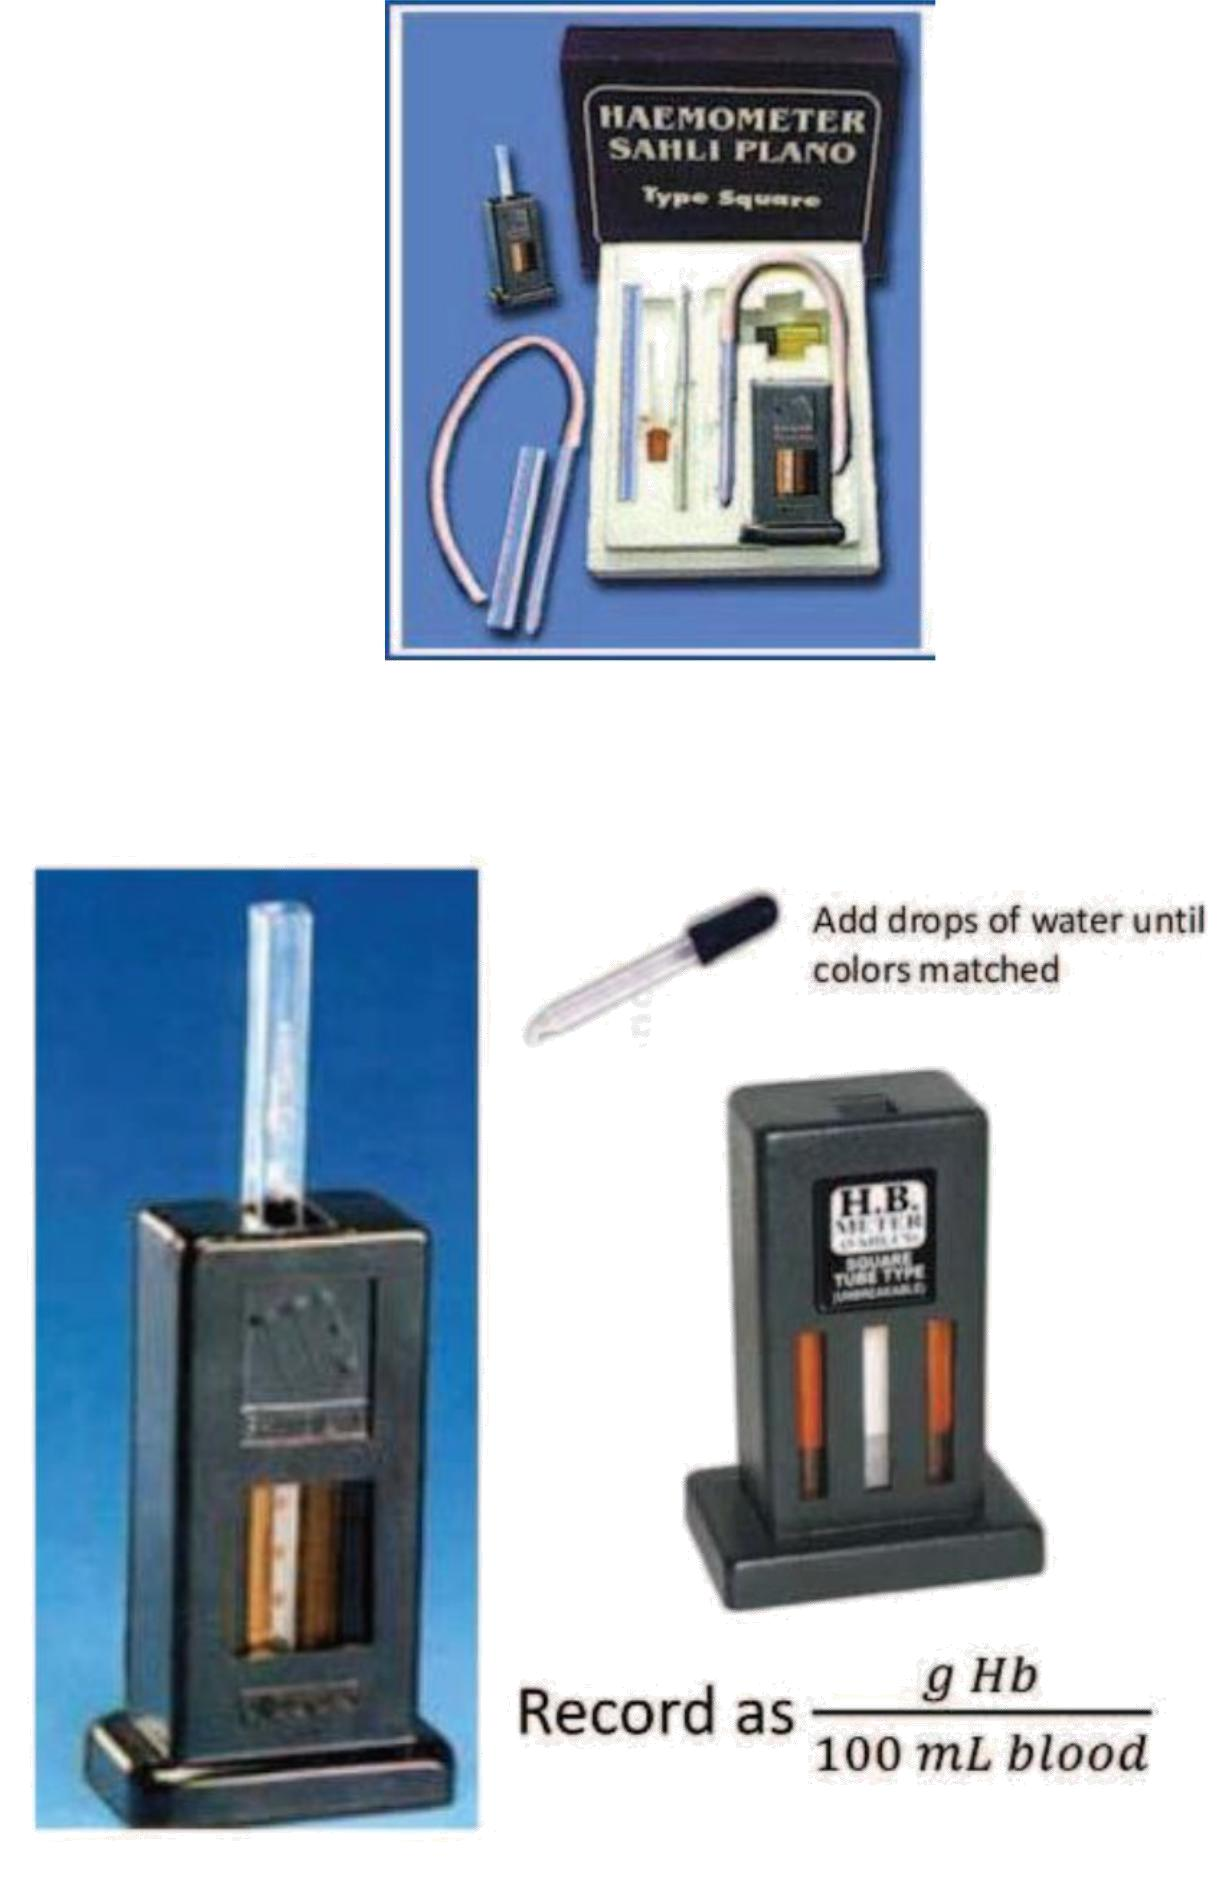
\includegraphics[scale=.25]{./hb.jpg}
									\label{hb}
									\caption*{\textbf{Sahli's Hemoglobinometer}}
								\end{figure}
								}
								To estimate the hemoglobin content of the blood by Sahli’s acid hematin method.
								\section*{Apparatus Required}
								Sahli’s Hemoglobinometer, Hemoglobin pipette, $\frac{N}{10}$ HCl, Distilled water, Glass stirrer, Dropper, Lancet, Spirit and Cotton.
								\section*{Principle}
								The amount of hemoglobin in the blood can be estimated by converting a known volume of blood into acid hematin solution and matching the color of the acid hematin solution with that of the standard colour.
								\section*{Description Of The Apparatus}
								The hemoglobinometer is a rectangular cubic box consisting of a central compartment to accommodate the ‘Hemoglobin tube’ and two yellow brown coloured cylindrical rods on either side as comparators. The Hb tube is graduated in percentage on one side and in gram percentage on the other side.

								The hemoglobin pipette has a single mark on the stem which corresponds to 0.02 ml or 20 cubic mm. A glass stirrer is provided for thorough mixing while diluting acid hematin solution.
								\section*{Procedure}
								\begin{enumerate}
									\item{Fill the hemoglobin tube with $\frac{N}{10}$ HCl upto its lowest mark (2 $g$\%).}
									\item{Prick the finger under aseptic precautions to form an adequate drop of blood and suck blood into the hemoglobin pipette upto 20 $mm^{3}$mark.}
									\item{Gently wipe exterior of the tip of the pipette.}
									\item{Insert the pipette into the hemoglobin tube containing $\frac{N}{10}$ HCl and blow out the blood. Rinse the pipette 2 or 3 times with the acid present in the tube.}
									\item{Wait for 10 minutes for the formation of acid hematin.}
									\item{Then, dilute the acid hematin by adding distilled water drop by drop and mix with the stirrer.}
									\item{Continue dilution till its color matches with that of the standards on either side.}
									\item{While matching, always take care to raise the stirrer above the level of the solution. Never take the stirrer out of the tube.}
									\item{Note down the final reading. (Lower meniscus).}
								\end{enumerate}
								\section*{Result}
								The Hb content of the given sample of blood is $\rule{5cm}{0.1cm}$ $g$\%
								\section*{Questions}
								\begin{enumerate}
									\item{What are the other methods used to estimate Hb content of blood?}
									\item{Which is the most reliable method for estimation of Hb?}
									\item{What are the different types of normal Hb in adults?}
									\item{Mention the names of abnormal hemoglobin.}
									\item{What are the differences between adult Hb \& fetal Hb?}
									\item{What are the different RBC indices? What are their clinical significance?}
								\end{enumerate}
								%-----}}}
								%-------BloodGrouping---{{{

								\chapter*{\centering Blood Grouping \& Typing}
								\begin{tabular}{p{5in} p{1in}}
									\textbf{Exp No:}  & \textbf{Date:}\\
								\end{tabular}

								\section*{Aim}

								\addfig{%
									\begin{figure}[h]
										\centering
										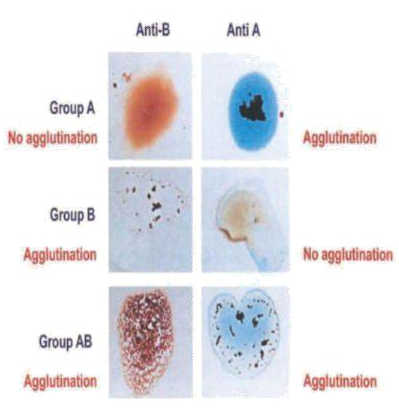
\includegraphics[scale=1.2]{./bloodGrouping.jpg}
										\label{bloodGrouping}
										\caption*{\textbf{Blood Groups Showing Agglutination}}
									\end{figure}
									}
									To determine uhe ABO blood group and Rh type of the given blood sample.
									\section*{Apparatus Required}
									Lancet, spirit, cotton, normal saline, clean white porcelain tile, glass marking pencil, anti-A serum, anti-B serum, anti-D serum, small sticks for mixing, glass slides, microscope.
									\section*{Principle}
									Determination of blood group is done by using specific agglutinins (antibodies), to confirm the presence or absence of corresponding agglutinogen (antigens) on the surface of the red blood cells.
									\section*{Procedure}
									\begin{enumerate}
										\item{Divide the porcelain tile into four columns with a marking pencil.}
										\item{Mark the columns as A, B, Rh and Control}
										\item{Take1ml of normal saline in a test tube.}
										\item{Prick the finger with the lancet under aseptic conditions.}
										\item{Mix 3-5 drops of blood with the saline to obtain a suspension of red blood cells.}
										\item{Add a drop each of anti-A, anti-B, anti-D sera and saline to the respective columns.}
										\item{Place a drop of the red cell suspension adjacent to the anti-sera in the respective columns.}
										\item{Mix the anti-sera and red cell suspension by using separate sticks.}
										\item{Wait for few minutes and observe the agglutination (clumping).}
										\item{Compare it with the saline standard.}
										\item{Record your findings.}
										\item{If there is doubt regarding agglutination, confirm it under the microscope.}
									\end{enumerate}
									\section*{Result}
									The blood group of the subject is $\rule{5cm}{0.1cm}$
									\section*{Questions}
									\begin{enumerate}
										\item{State Landsteiner’s law.}
										\item{What is cross-matching of blood?}
										\item{What is the preservative used to store blood in the blood bank?}
										\item{What are the clinical applications of blood grouping and Rh typing?}
										\item{What are the minor blood groups?}
										\item{What is the concept of universal donor/ universal recipient?}
										\item{What are the indications and hazards of blood transfusion?}
										\item{What are the differences between ABO system and Rh system?}
									\end{enumerate}
									%---------------}}}
									%----BleedingTime---{{{

									\chapter*{\centering Estimation Of Bleeding Time}
									\begin{tabular}{p{5in} p{1in}}
										\textbf{Exp No:}  & \textbf{Date:}\\
									\end{tabular}
									\addfig{%
										\begin{figure}[h]
											\centering
											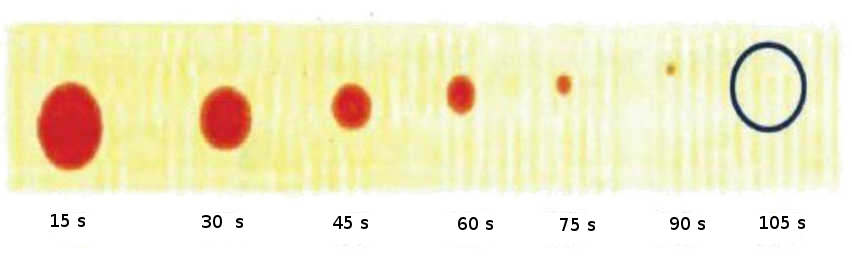
\includegraphics[scale=.5]{./bleedingTime.jpg}
											\label{bleedingTime}
											\caption*{\textbf{Estimation Of Bleeding Time}}
										\end{figure}
										}

										\section*{Aim}
										To determine the bleeding time by Duke’s method
										\section*{Apparatus Required}
										Filter paper, lancet, spirit, cotton swabs \& stop watch.	
										\section*{Principle}
										The time interval between skin puncture and spontaneous, unassisted stoppage of bleeding is called bleeding time. It is a test for assessing the function of platelets and integrity of capillaries.
										\section*{Procedure}
										\begin{enumerate}
											\item{Clean the tip of the finger with spirit and cotton and allow the finger to dry.}
											\item{Make a good deep finger prick with the lancet to get free flowing blood.}
											\item{Do not squeeze the finger.}
											\item{Immediately start the stopwatch.}
											\item{Gently touch the puncture site with a clean filter paper every 15 seconds.}
											\item{Repeat this step until no further blood spot appears on the filter paper.}
											\item{Observe that successive spots are smaller in size.}
											\item{Count the number of blood spots including the dry spot on the filter paper and divide it by 2 to get the bleeding time in minutes.}
											\item{Normal bleeding time by Duke’s method is 2-5minutes.}
										\end{enumerate}
										\section*{Result}
										The bleeding time determined by Duke’s method is $\rule{5cm}{0.1cm}$
										\section*{Questions}
										\begin{enumerate}
											\item{Define bleeding time.}
											\item{What are the other methods to determine the bleeding time?}
											\item{What is hemostasis?}
											\item{What is the role of platelets in hemostasis?}
											\item{What is the normal platelet count? What do you mean by thrombocytosis?}
											\item{Name few conditions where bleeding time is prolonged?}
											\item{What is Thrombocytopenic purpura? Comment on the clotting time in this condition.}
										\end{enumerate}
										%------------------------}}}
										%------------ClottingTime---{{{
										\chapter*{\centering Estimation Of Clotting Time}
										\begin{tabular}{p{5in} p{1in}}
											\textbf{Exp No:}  & \textbf{Date:}\\
										\end{tabular}
										\section*{Aim}

										\addfig{%
											\begin{figure}[h]
												\centering
												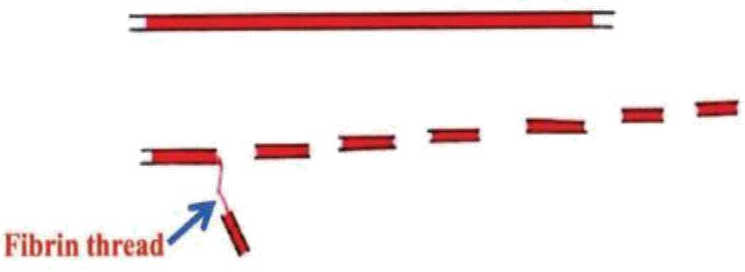
\includegraphics[scale=.5]{./clottingTime.jpg}
												\label{clottingTime}
												\caption*{\textbf{Estimation Of Clotting Time}}
											\end{figure}
											}
											To determine the clotting time of blood by Wright’s capillary glass tube method.
											\section*{Apparatus Required}
											Capillary glass tube, lancet, spirit, cotton swabs \& stop watch.
											\section*{Principle}
											When blood comes in contact with glass surface, the coagulation pathway gets activated.
											The time taken for the formation of insoluble fibrin thread(blood clot) is called clotting time.
											\section*{Procedure}
											\begin{enumerate}
												\item{Clean the tip of the ring finger with spirit and allow the finger to dry.}
												\item{Make a good deep finger prick with the lancet to get free flowing blood.}
												\item{Do not squeeze the finger.}
												\item{When a blood drop of optimum size has formed, gently place the end of the capillary tube in the drop such that the other end of the tube is at a lower level.}
												\item{Blood enters readily into the tube by capillary action.}
												\item{Start the stop watch.}
												\item{Hold the capillary tube with blood between the palms to maintain it at body temperature.}
												\item{After 2 minutes, break a small bit of capillary tube at its end and check for the formation of fibrin thread.}
												\item{Repeat it every 30 seconds until the appearance of insoluble fibrin thread between the broken ends of capillary tube and note the time.}
												\item{The appearance of the fibrin thread indicates that the blood has clotted.}
												\item{The total time taken for the formation of fibrin thread is recorded as the clotting time.}
												\item{Normal clotting time by this method is 2-8 minutes.}
											\end{enumerate}
											\section*{Result}

											The clotting time determined by Wright's capillary glass is $\rule{5cm}{0.1cm}$
											\section*{Questions}
											\begin{enumerate}
												\item{Define clotting time.}
												\item{What are the other methods used to determine the clotting time?}
												\item{Name the conditions in which clotting time is prolonged.}
												\item{What is haemophilia? Comment on the clotting time in this condition.}
												\item{What is clot retraction time?}
												\item{Name the Vitamin K dependent coagulation factors.}
												\item{What is an anticoagulant? Mention some invivo and invitro anticoagulants.}
												\item{Name the proteins involved in fibrinolytic system.}
											\end{enumerate}
											%--------}}}
											%-----ESR------{{{

											\chapter*{\centering Estimation Of Erythrocyte Sedimentation Rate}
											\begin{tabular}{p{5in} p{1in}}
												\textbf{Exp No:}  & \textbf{Date:}\\
											\end{tabular}
											\section*{Aim}
											To determine the Erythrocyte Sedimentation Rate of the given blood sample.
											\section*{Apparatus Required}

											\addfig{%
												\begin{figure}[h]
													\centering
													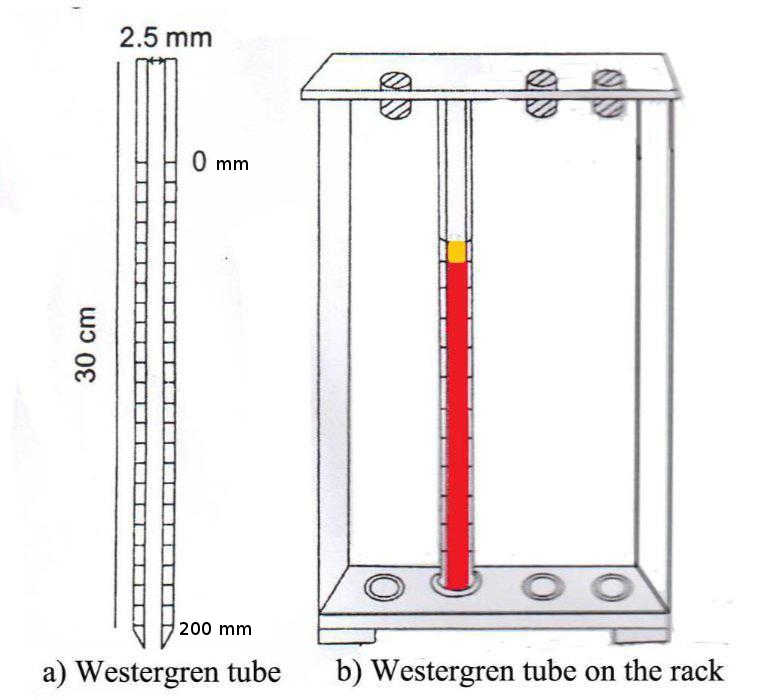
\includegraphics[scale=.5]{./esr.jpg}
													\label{esr}
													%\caption*{\textbf{Estimation Of Clotting Time}}
												\end{figure}
												}
												Westergren’s pipette and stand, syringe with needle and 3.8\% sodium citrate solution (anticoagulant)

												\section*{Principle}
												If blood treated with anticoagulant is allowed to stand in a tube placed vertically, the RBCs settle down gradually to the bottom since their specific gravity (1.093) is greater than that of the plasma (1.030).
												The rate  at  which the  RBCs settle down is called as Erythrocyte Sedimentation
												Rate.

												\section*{Procedure}
												\textbf{Westergren’s method:}\newline
												\begin{enumerate}	
													\item{Westergren’s pipette (tube) which is used for this procedure is open at both ends and is graduated in $mm$ from 0-200 with a bore diameter of 2.5$mm$.}
													\item{A sterile solution of 3.8\% sodium citrate is used as an anticoagulant.}
													\item{In a clean dry syringe, draw 2ml of blood from the antecubital vein under aseptic precautions and mix with 0.4ml of 3.8\% sodium citrate solution in a plastic  container with its lid closed.}
													\item{Fill the Westergren’s pipette with blood by sucking, after placing the tip of the finger over the top of the pipette to control the flow of blood into and out of it, or with a rubber bulb.}
													\item{Bring the blood column to exact zero mark.}
													\item{Keeping the finger (or the rubber bulb) over the pipette, transfer it to the Westergren stand by firmly pressing its lower end into the rubber cushion. Now.}
													\item{slip the upper end of the pipette under the screw cap.}
													\item{After an hour, note the $mm$ of clear plasma above the red cells.}
												\end{enumerate}
												\section*{Result}
												Erythrocyte Sedimentation Rate of the given blood sample is $\rule{5cm}{0.1cm}$ $mm$ in first hour.
												\section*{Questions}
												\begin{enumerate}
													\item{What is ESR?}
													\item{What are the 3 stages by which sedimentation of red cells occur?}
													\item{What are the other methods of estimating ESR?}
													\item{What are the advantages and disadvantages of Westergren method?}
													\item{What are the advantages and disadvantages of Wintrobe method?}
													\item{Can you use oxalate mixture in Westergren method and citrate in Wintrobe method?}
													\item{What are the factors determining ESR?}
													\item{What is rouleaux formation?}
													\item{Why is ESR reading taken after one hour?}
													\item{What is the normal ESR in males and females?}
													\item{Why is the ESR higher in females than that of males?}
													\item{What is the clinical significance of ESR?}
													\item{Mention some physiological and pathological conditions in which ESR is increased / decreased?}
													\item{What is zeta potential?}
												\end{enumerate}
												%------------------------}}}
												%---PackedCellVolume-{{{

												\chapter*{\centering Packed Cell Volume}
												\begin{tabular}{p{5in} p{1in}}
													\textbf{Exp No:}  & \textbf{Date:}\\
												\end{tabular}

												\section*{Aim}

												\addfig{%
													\begin{figure}[h]
														\centering
														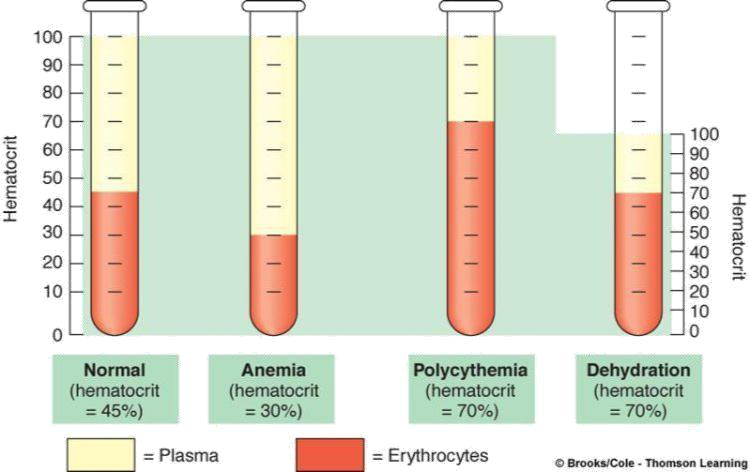
\includegraphics[scale=.5]{./pcv.jpg}
														\label{pcv}
														\caption*{\textbf{Estimation Of Packed Cell Volume }}
													\end{figure}
													}
													To determine the packed cell volume of the given blood sample.
													\section*{Apparatus Required}
													Centrifuge, Hematocrit tube (Wintrobe tube), Pasteur pipette, syringe with needle and double oxalate or EDTA (anticoagulant).
													\section*{Principle}
													When the blood is mixed with an anticoagulant and centrifuged in a hematocrit tube, the red blood corpuscles settle down at the bottom. The ratio of the volume of the settled red blood cells to that of whole blood in the hematocrit tube is called the packed cell volume or the hematocrit. A thin grey-white layer of white cells at the top of the red blood cell column is called the buffy coat layer.
													Hematocrit measures the percentage of volume of the packed red cells. It is used to diagnose and classify the various types of anemia, along with other red blood cell indices.
													\section*{Procedure}
													\textbf{Wintrobe's Method:}\newline
													\begin{enumerate}
														\item{Wintrobe’s tube is a thick walled cylindrical tube, 11$cm$ in length with an internal bore of 3$mm$. The tube is graduated from 0 to 10$cm$(100 $mm$) both in the ascending and descending order on either sides. The marking 0 – 10 from above downwards is used for ESR and the marking 0-10 from below upwards is used for reading PCV.}
														\item{In a clean dry syringe, 2ml of blood is drawn from the antecubital vein under aseptic precautions and transferred to a container with anticoagulant.}
														\item{The anticoagulated blood is then filled in the hematocrit tube from below upwards upto the mark 10 using the Pasteur pipette.}
														\item{The tube is centrifuged at a rate of 3000 rpm for a period of 30 minutes.}
														\item{At the end of 30 minutes, take the reading of upper level of packed red cell column.}
													\end{enumerate}
													\section*{Result}
													The packed cell volume or the hematocrit value of the given blood sample is $\rule{2cm}{.1cm}$\%
													\section*{Questions}
													\begin{enumerate}
														\item{Define PCV.}
														\item{What is the clinical significance of PCV?}
														\item{What is the normal range of PCV in males and females?}
														\item{What is the ideal anti-coagulant used and why?}
														\item{What is the difference between arterial and venous blood hematocrit?}
													\end{enumerate}
													%-----------------}}}
													%---------OsmoticFragility---{{{
													\chapter*{\centering Osmotic Fragility}
													\begin{tabular}{p{5in} p{1in}}
														\textbf{Exp No:}  & \textbf{Date:}\\
													\end{tabular}

													\section*{Aim}

													\addfig{%
														\begin{figure}[h]
															\centering
															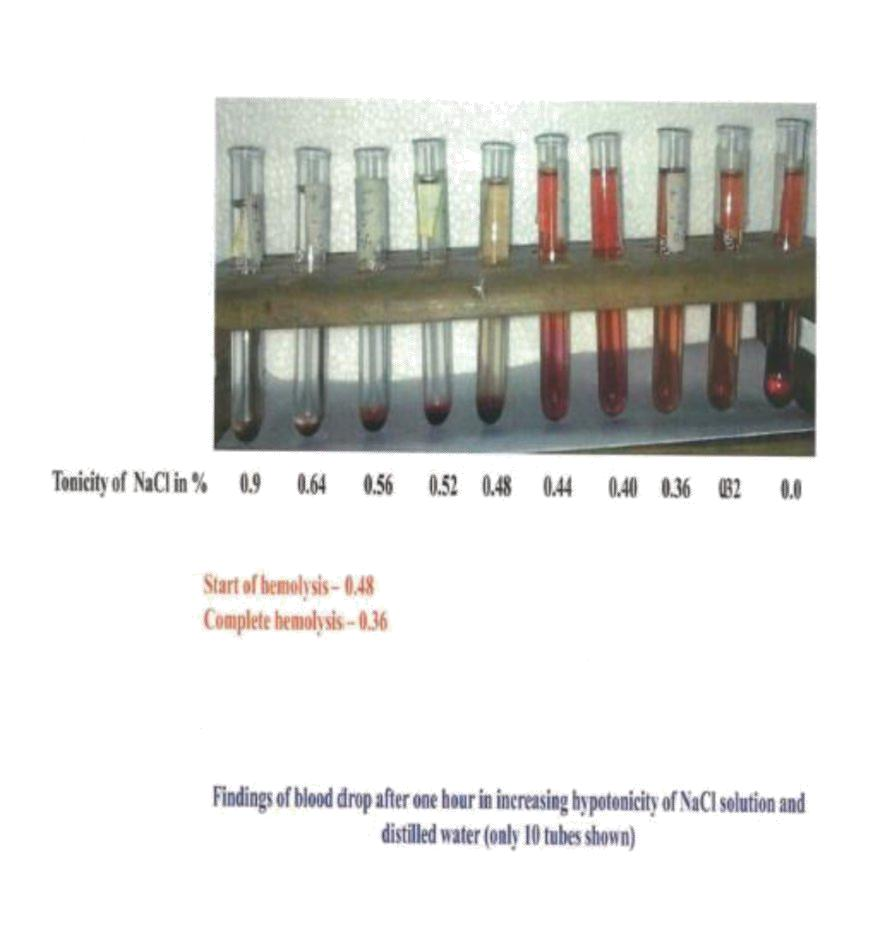
\includegraphics[scale=.5]{./osmoticFragility.jpg}
															\label{osmoticFragility}
															\caption*{\textbf{Estimation Of Osmotic Fragility}}
														\end{figure}
														}
														To determine the osmotic fragility of red blood cells in the given sample of blood.
														\section*{Apparatus Required}
														Test tubes with rack, anticoagulated blood, NaCl, distilled water.
														\section*{Principle}
														The normal red blood cells can remain suspended in 0.9\% sodium chloride solution (normal saline) for hours without any change in their size \& shape. But when they are placed in decreasing strengths of hypotonic sodium chloride solutions they imbibe water due to osmosis and finally burst releasing the hemoglobin pigment in the medium.
														\section*{Procedure}
														\begin{enumerate}
															\item{Sodium chloride solution of 1\% tonicity is prepared by dissolving 1 gram of NaCl in 100ml of distilled water.}
															\item{Arrange the test tubes in the rack and number them serially from 1 to 12.}
															\item{Prepare solutions of increasing hypotonicity by mixing required number of drops of 1\% NaCl solution and distilled water in the test tubes as given in the table.}
															\item{Use separate droppers for saline solution and distilled water.}
															\item{Note that the tube No.1 contains normal saline (0.9\% approximately) – Isotonic with plasma while tube No.12 contains distilled water.}
															\item{Draw 2ml of venous blood and treat it with anticoagulant in a test tube.}
															\item{Add one drop of blood into each of the above 12 tubes.}
															\item{Invert each tube gently once to mix blood with saline.}
															\item{Leave the test tubes undisturbed for one hour. Then observe the extent of hemolysis in each tube by holding the rack at eye level, with a white paper sheet behind it.}
														\end{enumerate}

														\begin{center}
															\csvautotabular{./osmoticFragility.csv}
														\end{center}
														\section*{Intrepretation}

														\begin{itemize}
															\item{Test tube with partial hemolysis shows a supernatant fluid with pink colour proportionate to the degree of hemolysis and a lower layer of sedimented red cells at the bottom of the tube.}
															\item{Test tube with complete hemolysis shows a clear homogeneously pink solution with no cells at the bottom.}
															\item{Test tube with no hemolysis shows a clear colourless supernatant solution with a layer of sedimented red cells at the bottom of the tube}
														\end{itemize}
														\section*{Result}
														Hemolysis begins in $\rule{4cm}{.1cm}$\% of NaCl solution.\newline
														Hemolysis is complete in $\rule{4cm}{.1cm}$\% of NaCl solution.
														\section*{Questions}
														\begin{enumerate}
															\item{What is the normal range of osmotic fragility of red cells?}
															\item{What is osmosis?}
															\item{What do you mean by hypo/hyper tonicity?}
															\item{Define fragility.}
															\item{What happens to red cells when they are placed in isotonic, hypotonic and hypertonic solutions?}
															\item{Name some conditions which increase / decrease the osmotic fragility of the RBC.}
															\item{What are the advantages of the shape of red blood cells?}
														\end{enumerate}	
														%----------------------------}}}
														%--------------------------------SpecificGravity------------------------------{{{


														\chapter*{\centering Specific Gravity}

														\begin{tabular}{p{5in} p{1in}}
															\textbf{Exp No:}  & \textbf{Date:}\\
														\end{tabular}

														\section*{Aim}
														To determine the specific gravity of the given blood sample by using “Copper sulphate falling drop method”.

														\section*{Apparatus Required}

														\addfig{%
															\begin{figure}[h]
																\centering
																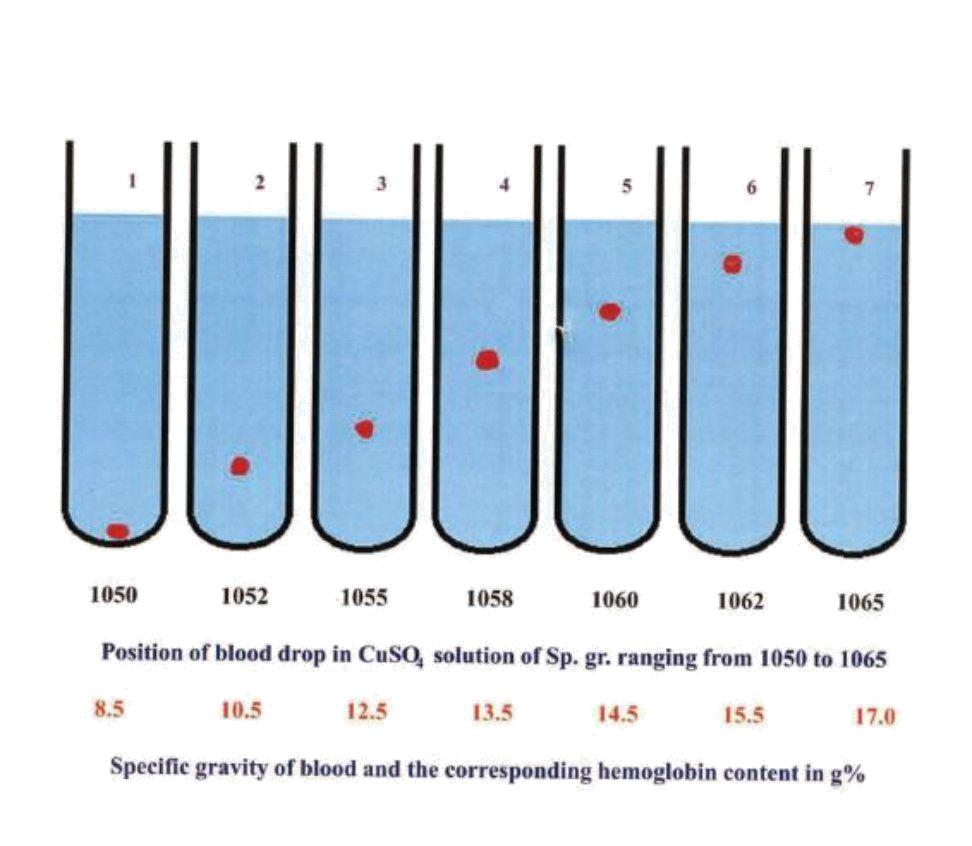
\includegraphics[scale=.5]{./specificGravity.jpg}
																\label{specificGravity}
																\caption*{\textbf{Determination Of Specific Gravity}}
															\end{figure}
															}
															Test tubes with rack, distilled water, anticoagulated blood, copper sulphate crystals (CuSO$_4$.5H$_2$O), beaker, measuring jar, Pasteur pipette
															\section*{Principle}
															The specific gravity of blood is determined by comparing the specific gravity of one drop of blood with that of copper sulphate solution of known specific gravity.
															\section*{Procedure}
															\begin{enumerate}
																\item{Stock solution of copper sulphate is prepared by dissolving 159 $g$ of CuSO$_4$.5H$_2$O in 1 liter of distilled water. The specific gravity of this stock solution is 1100.}
																\item{Standard copper sulphate solutions of known specific gravity are prepared by mixing specific quantity of stock solution and distilled water as shown in table and label the test tubes.}
																\item{Arrange the test tubes in rack in order of increasing specific gravity from left to right in test tube rack.}
																\item{Draw 2ml of venous blood and treat it with the anticoagulant in a test tube.}
																\item{Using Pasteur pipette a drop of blood is delivered into the middle test tube (no.4) from a height of about 1$cm$ above the surface of the copper sulphate solution so that it doesn’t touch the walls of the test tube.}
																\item{The drop sinks to about 2-3$cm$, and loses its momentum in 3-4 seconds. The drop then behaves according to its specific gravity; observe its behaviour during the next 15 seconds.}
																\item{If the specific gravity of blood drop is greater than that of the solution, the drop sinks to the bottom; if it is less than that of the solution, it rises to the surface and if it is the same as that of the solution, it becomes stationary and floats in the middle of the solution.}
																\item{If the drop continues to sink in test tube no.4, try with higher specific gravity solution; if it begins to rise, try with the lower specific gravity solution till you come to a solution where the drop remains in the middle of the solution.}
																\item{The whole observation has to be made in each step within 15 seconds.}
																\item{The tube in which the blood drop remains suspended in the middle of the tube for at least 15 seconds is noted and the specific gravity mentioned on the tube is read and recorded.}

															\end{enumerate}
															\begin{center}
																\csvautotabular{./specificGravity.csv}
															\end{center}
															\section*{Result}
															The specific gravity of the given blood sample is $\rule{4cm}{.1cm}$.
															\section*{Questions}
															\begin{enumerate}
																\item{Define specific gravity.}
																\item{What is the normal specific gravity of blood, plasma, serum and red blood cells?}
																\item{Why is copper sulphate solution used in this experiment?}
																\item{Why should the observation be made within 15 seconds?}
																\item{Enlist the physiological and pathological conditions in which the specific gravity of blood is increased and decreased.}
																\item{What are the clinical applications of this method? }
															\end{enumerate}
															%----------------------------------------------------------------------------}}}
															%-----------}}}

															\part{Clinical Physiology}

															\chapter*{\centering General Examination}

															\begin{tabular}{p{5in} p{1in}}
																\textbf{Exp No:}  & \textbf{Date:}\\
															\end{tabular}
															A thorough general examination is done before any systemic examination. Vital information such as name, age, sex, height, weight, occupation and address of the individual are recorded. The subject is comfortably seated. The room is well illuminated. It is always preferable to examine under good day light. The examiner should always be on the right side of the subject while examining.
															\section*{The following observations are recorded:}
															\subsection*{Level Of Consciousness}
														\addfig{%
															\begin{figure}[h]
																\begin{subfigure}[t]{.3\textwidth}
																	\centering
																	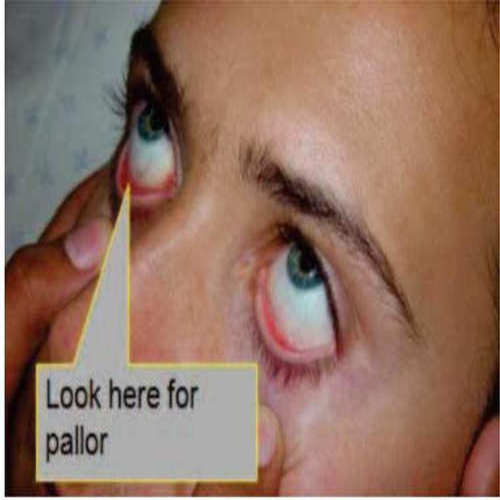
\includegraphics[width=\textwidth]{./clinicalPhysioPic/pallor1.jpg}
																	\subcaption{Site Of Examination of Pallor} 
																	\label{lpc}
																\end{subfigure}
																\begin{subfigure}[t]{.3\textwidth}
																	\centering
																	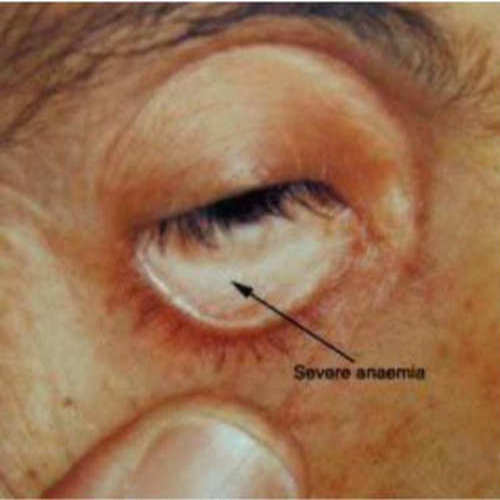
\includegraphics[width=\textwidth]{./clinicalPhysioPic/pallor2.jpg}
																	\caption{Lower Palpabral Conjunctiva In Severe Anemia}
																	\label{pallor}
																\end{subfigure}
																\begin{subfigure}[t]{.3\textwidth}
																	\centering
																	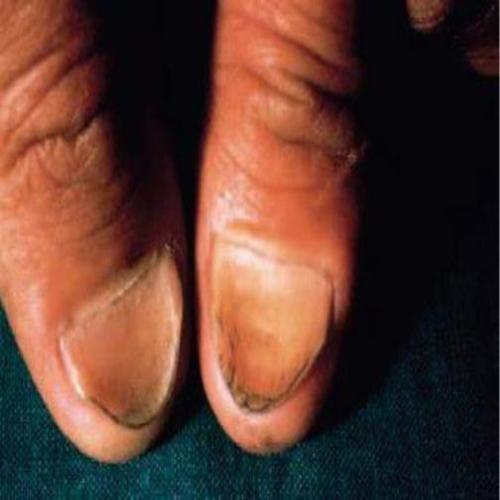
\includegraphics[width=\textwidth]{./clinicalPhysioPic/koilonychia.jpg}
																	\caption{Koilonychia}
																	\label{koilonychia}
																\end{subfigure}
																\begin{subfigure}[t]{.3\textwidth}
																	\centering
																	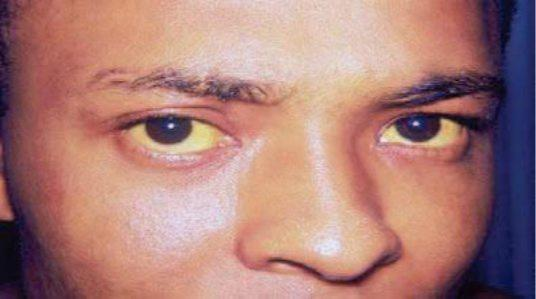
\includegraphics[width=\textwidth]{./clinicalPhysioPic/jaundice.jpg}
																	\caption{Icterus}
																	\label{icterus}
																\end{subfigure}
																\begin{subfigure}[t]{.3\textwidth}
																	\centering
																	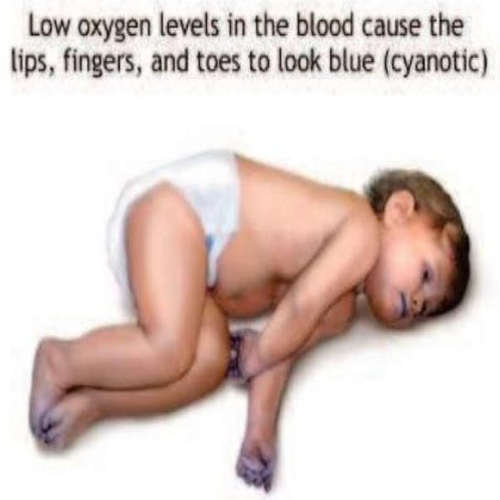
\includegraphics[width=\textwidth]{./clinicalPhysioPic/cyanosis4-0.jpg}
																	\caption{Cyanosis}
																	\label{cyanosis1}
																\end{subfigure}
																\begin{subfigure}[t]{.3\textwidth}
																	\centering
																	
\includegraphics[width=\textwidth]{./clinicalPhysioPic/cyanosis4-1.jpg}
																	\caption{Cyanosis}
																	\label{cyanosis2}
																\end{subfigure}
																\begin{subfigure}[t]{.3\textwidth}
																	\centering
																	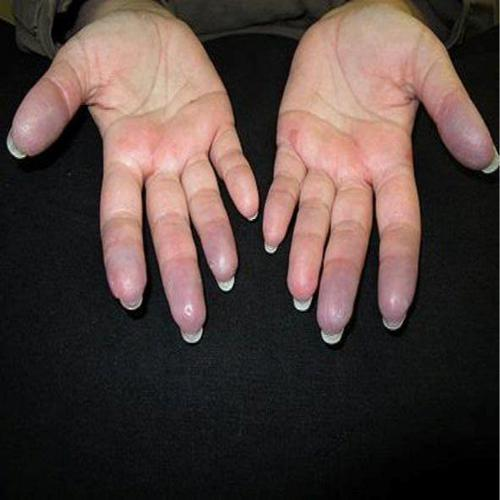
\includegraphics[width=\textwidth]{./clinicalPhysioPic/cyanosis4-2.jpg}
																	\caption{Cyanosis}
																	\label{Cyanosis3}
																\end{subfigure}
																\begin{subfigure}[t]{.3\textwidth}
																	\centering
																	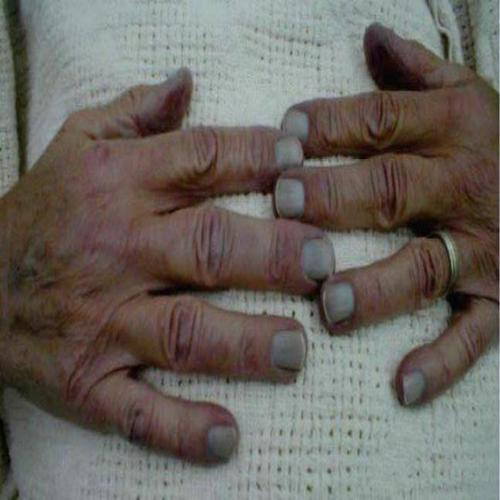
\includegraphics[width=\textwidth]{./clinicalPhysioPic/cyanosis4-3.jpg}
																	\caption{Cyanosis}
																	\label{Cyanosis4}
																\end{subfigure}
																\begin{subfigure}[t]{.3\textwidth}
																	\centering
																	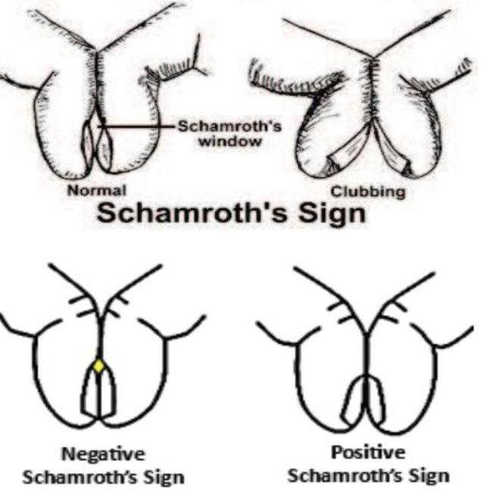
\includegraphics[width=\textwidth]{./clinicalPhysioPic/clubbing3-0.jpg}
																	\caption{Clubbing}
																	\label{Clubbing1}
																\end{subfigure}
																\begin{subfigure}[t]{.3\textwidth}
																	\centering
																	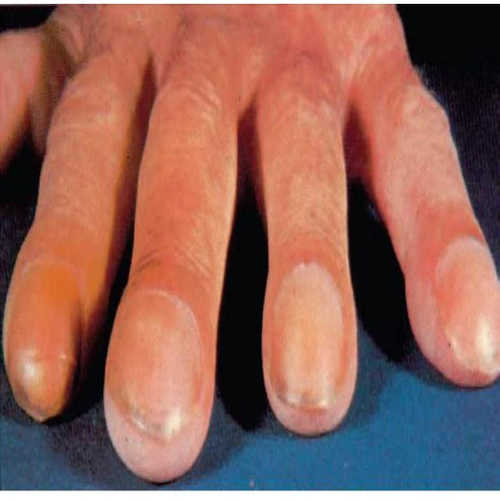
\includegraphics[width=\textwidth]{./clinicalPhysioPic/clubbing3-1.jpg}
																	\caption{Clubbing}
																	\label{Clubbing2}
																\end{subfigure}
																\begin{subfigure}[t]{.3\textwidth}
																	\centering
																	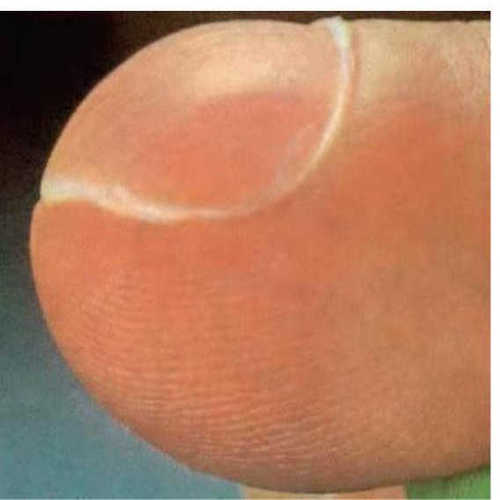
\includegraphics[width=\textwidth]{./clinicalPhysioPic/clubbing3-2.jpg}
																	\caption{Clubbing}
																	\label{Clubbing3}
																\end{subfigure}
																\begin{subfigure}[t]{.3\textwidth}
																	\centering
																	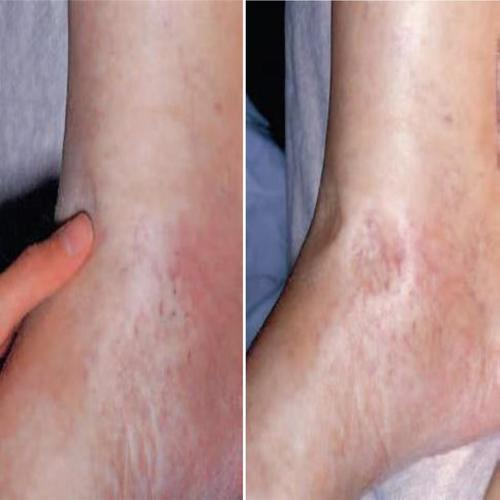
\includegraphics[width=\textwidth]{./clinicalPhysioPic/pittingPedalEdema.jpg}
																	\caption{Pedal Edema}
																	\label{PedalEdema}
																\end{subfigure}
																\caption*{General Examination}
															\end{figure}
															}
															The level of consciousness can be clear sensorium, drowsiness, stupor, semicoma and coma.
															\subsection*{Orientation To Time, Place And Person}
															Ask about the day, date, month, year and time of day. Subject should know where they are (e.g. home or hospital) Similarly test his orientation towards person.
															\subsection*{Body Build And Nourishment}
															Build refers to skeletal frame work and nourishment refers to muscular bulk. It should be observed whether he is well / moderately / thin built and nourished.
															\subsection*{Temperature}
															Recorded by a clinical thermometer.\newline
															\begin{itemize}
																\item{\textbf{Method of recording temperature:}}

																	Do not touch the bulb of the thermometer. Shake down the mercury column into the bulb. Keep it under the tongue with the mouth closed for one minute before reading the temperature.
																\item{\textbf{Sites of recording temperature:}}
																	\begin{itemize}%Sites of recording temperature:]
																		\setlength\itemsep{.5em}
																		\item{Mouth ( 36.6$^{\circ}$C to 37.2C$^{\circ}$C )}
																		\item{Axilla ( 0.5 $^{\circ}$C lower than oral temperature )}
																		\item{Rectum ( 0.5 $^{\circ}$C higher than oral temperature – Closer to core temperature )}
																	\end{itemize}
															\end{itemize}

															\subsection*{Pallor}
															Pallor of the skin and mucous membrane.
															\begin{itemize}
																\item{\textbf{Areas to look for pallor}}
																	\begin{itemize}
																		\item{Lower palpebral conjunctiva}
																		\item{Instruct the subject to look up and retract the lower lid to see the palpebral conjunctiva}
																		\item{Dorsum of tongue}
																		\item{Mucous membrane of oral cavity}
																		\item{Nail bed}
																		\item{Skin over palm and sole}
																	\end{itemize}

																\item{\textbf{Conditions where pallor is seen}}
																	\begin{itemize}
																		\item{Anemia – Reduced count of RBCs / Hb content in blood}
																		\item{Shock}
																	\end{itemize}
															\end{itemize}
															\subsection*{Jaundice ( Icterus )}
															Yellowish discoloration of the sclera, skin and the mucous membrane due to presence of excess bilirubin in blood of more than 2 $mg$\%
															\begin{itemize}
																\item{\textbf{Areas to look for jaundice}}
																	\begin{itemize}
																		\item{Bulbar conjunctiva of both eyes – Upper sclera}
																			(Instruct the subject to look down and retract the upper lid to view the sclera)
																		\item{Mucus membrane of oral cavity}
																			(especially the undersurface of tongue and floor of mouth)
																		\item{Nail bed}
																		\item{Skin}
																	\end{itemize}
																\item{\textbf{Causes of yellowish discoloration of skin}}
																	\begin{itemize}
																		\item{Jaundice, Carotenemia, Hemochromatosis}
																	\end{itemize}

																\item{\textbf{Hypercarotenemia occurs in}}
																	\begin{itemize}
																		\item{People who eat large quantity of raw carrots and tomatoes}
																		\item{Hypothyroidism.}
																	\end{itemize}
															\end{itemize}
															\subsection*{Cyanosis}
															It is the bluish discoloration of the skin and mucous membrane due to an increased quantity of reduced hemoglobin concentration of more than 5 gm in 100 ml of blood.
															\begin{itemize}
																\item{\textbf{Areas to look for cyanosis:}}
\begin{itemize}
\item{Lips}
\item{Tongue}
\item{Mucous membrane over the Palate}
\item{Conjunctiva}
\item{Tip of the nose and ear lobules}
\item{Extremities (fingers, toes and nail beds)}
																	\end{itemize}
																\item{\textbf{Types of Cyanosis:}}
\begin{itemize}
\item{	Central cyanosis}
\item{	Peripheral cyanosis}
\item{	Differential cyanosis}
\end{itemize}
\end{itemize}

\subsection*{Clubbing}
Bulbous enlargement of soft parts of the terminal phalanges with over curving of the nails both longitudinally and transversely.
\begin{itemize}
	\item{\textbf{Schamroth’s sign:}}
	\begin{itemize}
\item{When two fingers of both hands are held together with their nails facing each other, a diamond shaped space is seen. This space is lost in clubbing (Positive Schamroth’s sign).}
	\end{itemize}
\item{\textbf{Clubbing is seen in}}
	\begin{itemize}
\item{Bronchopulmonary diseases like bronchiectasis, lung abscess, empyema, chronic bronchitis and bronchogenic carcinoma}
\item{Cardiac diseases like congenital cyanotic heart disease and bacterial endocarditis}
\item{Gastro intestinal diseases like ulcerative colitis and liver cirrhosis}
\item{Endocrine disorders like acromegaly, thyrotoxicosis}
\item{Hereditary}
	\end{itemize}
\end{itemize}

\subsection*{Oedema}
It is the condition where there is accumulation of free fluid in the interstitial space. Pedal oedema is examined by pressing the skin and the tissue against the tibial bone just above the medial malleolus, sustaining the pressure for at least 15 seconds and releasing the pressure to look for pitting, if any. In bed ridden subjects oedema is examined by pressing over the presacral region.

\begin{itemize}
\item{\textbf{Types of oedema:}}
\begin{itemize}
\item{Pitting oedema – Heart failure, renal disease, hypoproteinemia}
\item{Non-pitting oedema – Myxoedema, filariasis}
\end{itemize}
\end{itemize}

\subsection*{Lymphadenopathy}
\begin{itemize}
	\item{\textbf{Group of nodes to be examined:}}
		\begin{itemize}
\item{Submental, submandibular, cervical, posterior auricular, occipital,  supraclavicular, axillary, inguinal and popliteal nodes.}
		\end{itemize}
\item{\textbf{Points to be noted while examining lymph nodes:}}
	\begin{itemize}
\item{Site, size, number, consistency (soft, firm or hard), tenderness, mobility, matted or discrete, fixity to skin, generalized or localized.}
	\end{itemize}
\item{\textbf{Examination of lymph nodes:}}
	\begin{itemize}
\item{Examiner should stand behind the sitting subject- Submental, submandibular, deep cervical nodes in the anterior triangle of neck}
\item{Examiner should stand in front of the sitting subject – deep cervical nodes in the posterior triangle of neck, posterior auricular and occipital nodes}
\item{Axillary nodes – sitting posture with abducted arm}
\item{Inguinal nodes – supine position with thigh flexed to 10$^{\circ}$}
\item{Popliteal nodes – Flex the knees and palpate deep into popliteal fossa}
	\end{itemize}
\end{itemize}

\subsection*{Questions}
\begin{enumerate}
\item{Where will you look for pallor?}
\item{What is cyanosis?}
\item{What are the types of Jaundice?}
\item{How do you detect clubbing?}
\item{What are the types of oedema and what are their causes?}
\item{What are the vital signs?}
\end{enumerate}
											    \end{document}
